\documentclass[compress, xelatex, 11pt, xcolor=svgnames, aspectratio=169,
	hyperref={
		bookmarks=true,
		unicode=true,
		colorlinks=true,
		pdftitle={Citacni software},
		plainpages=false,
		pdfauthor={Vojtech Zeisek},
		pdfsubject={Kratky uvod do citacniho software},
		pdfcreator={XeLaTeX},
		pdfkeywords={citace, reference, software, literatura},
		linkcolor=Crimson, % Navigační odkazy menu na stránkách a v navigačním menu
		anchorcolor=Magenta, % Nepoužívá se?
		citecolor=Magenta, % Nepoužívá se?
		filecolor=Magenta, % Nepoužívá se?
		menucolor=Magenta, % Nepoužívá se?
		urlcolor=DarkTurquoise, % Odkazy s \href a \url
		},
	url={hyphens, lowtilde} % Řádkové zlomy v dlouhých URL
	]{beamer}

% Fonts Linux Libertine
\usepackage{libertine}

% TeX logos
\usepackage{dtk-logos}

% Nastavení vzhledu
\usecolortheme{spruce}
\useinnertheme[shadow]{rounded}
\useoutertheme{shadow}

\setbeamertemplate{headline} {
	\hbox{%
		\begin{beamercolorbox}[wd=\paperwidth, ht=2.65ex, dp=1.5ex, right]{section in head/foot}
			\insertsectionnavigationhorizontal{\paperwidth}{\hskip0pt plus1fill}{\hskip0pt plus1fill}
			\end{beamercolorbox}%
		}
	\vskip 0pt
	}

\setbeamertemplate{footline} {
	\hbox{%
		\begin{beamercolorbox}[wd=0.333333\paperwidth, ht=2.25ex, dp=1ex, center]{author in head/foot}
			\usebeamerfont{author in head/foot}\insertshortauthor~(\insertshortinstitute)
		\end{beamercolorbox}%
		\begin{beamercolorbox}[wd=0.333333\paperwidth, ht=2.25ex, dp=1ex, center]{title in head/foot}
			\usebeamerfont{title in head/foot}\insertshorttitle
		\end{beamercolorbox}%
		\begin{beamercolorbox}[wd=0.333333\paperwidth, ht=2.25ex, dp=1ex, right]{date in head/foot}
			\usebeamerfont{date in head/foot}\insertshortdate{}\hspace*{2em}
			\insertframenumber{} / \inserttotalframenumber\hspace*{2ex} 
		\end{beamercolorbox}%
		}
	\vskip 0pt
	}

% Jazyk
\usepackage{polyglossia}
\setmainlanguage{czech}

% Quotes
\usepackage[autostyle=true]{csquotes}

% Titulka
\author{Vojtěch Zeisek}
\institute[PřF UK \& BÚ AV ČR]{Katedra botaniky PřF UK \& Botanický ústav AV ČR\\ \url{https://trapa.cz/cs}, \href{mailto:zeisek@natur.cuni.cz}{zeisek@natur.cuni.cz}}
\title{Citační software}
\subtitle{O~software, který vám pomůže a~usnadní práci}
\date{10. 11. 2023}
\titlegraphic{
\includegraphics[height=2cm]{logo.jpg}}

\begin{document}

\begin{frame}
	\titlepage
\end{frame}

\begin{frame}{Obsah}
	\tableofcontents
\end{frame}

\section{Obecně}

\begin{frame}{K~čemu to je~I}{Usnadnění jinak pracného udržování citací}
	\begin{itemize}
		\item V~každém odborném textu, včetně BP, musí být veškerá tvrzení vždy doložena citacemi (Usus, 1800).
		\item Jinak text neprojde (Obhajoba \& Komise, 2013).
	\end{itemize}
	\textbf{Literatura:}
	\begin{itemize}
		\item Usus, Obecný Odborný 1800. Psaní odborného textu. Journal of Understanding, \textbf{1}, 209--216.
		\item Obhajoba, Veřejná \& Komise Zkušební 2013. Hodnocení kvality. Journal of Acceptance \textbf{(2013)} 8--15.
	\end{itemize}
	\vfil
	\hrulefill
	\vfill
	Ručně to lze dělat dokud máte pár stránek textu, jednotky citací a~nebudete citace měnit a~nebudete měnit styl jejich zobrazení\ldots
\end{frame}

\begin{frame}{K~čemu to je~II}{Tvrzení musí být doložená\ldots}
	\begin{center}
		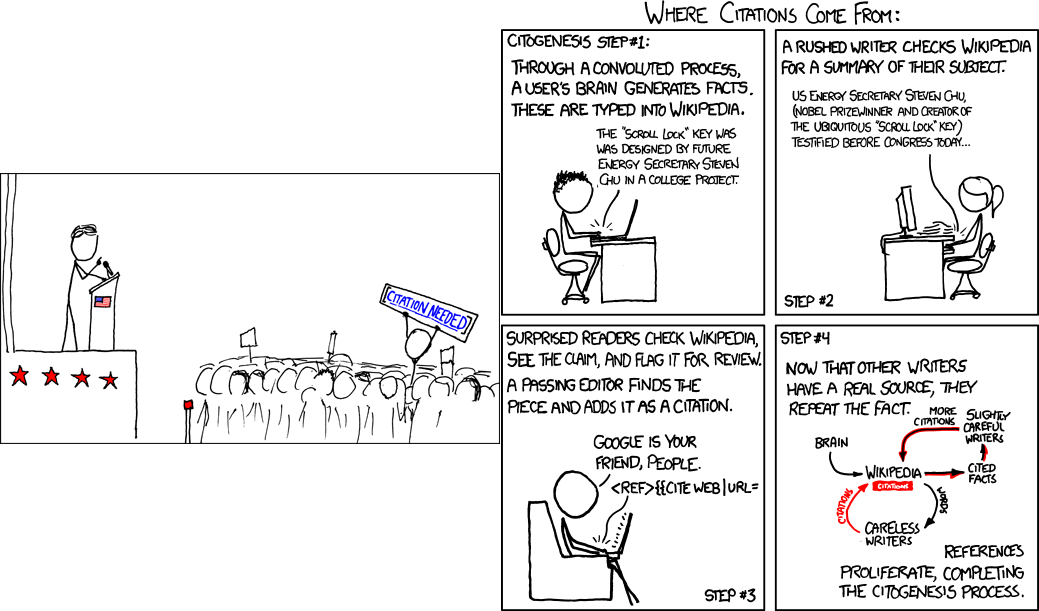
\includegraphics[height=6cm]{xkcd.png}
	\end{center}
	\begin{flushright}
		\url{https://xkcd.com/285/} a~\url{https://xkcd.com/978/}
	\end{flushright}
\end{frame}

\begin{frame}{K~čemu to je~III}
	\begin{itemize}
		\item V~každém odborném textu, včetně BP, musí být veškerá tvrzení vždy doložena citacemi$^{1}$.
		\item Jinak text neprojde$^{2}$.
	\end{itemize}
	\textbf{Literatura:}
	\begin{enumerate}
		\item Usus, OO. Psaní odborného textu. J. Understand. 1, 209--216 (1800).
		\item Obhajoba, V \& Komise Z. Hodnocení kvality. J. Accept. 213, 8--15 (2013).
	\end{enumerate}
	\vfill
	\hrulefill
	\vfill
	\textbf{Chcete to dělat ručně? Vážně?}
	\begin{itemize}
		\item Vše citované v~textu bude v~literatuře a~naopak\ldots?
		\item Budete mít stovky článků a~desítky stran textu\ldots?
		\item Vše bude mít jednotný styl\ldots?
		\item Udržíte pořádek když to~začnete měnit\ldots?
	\end{itemize}
\end{frame}

\begin{frame}[allowframebreaks]{Jaký citační software existuje --- výběr}
	\begin{itemize}
		\item \textbf{Zotero} --- multiplatformní, freeware, open-source, dostupný na~\url{https://www.zotero.org/}
		\item \textbf{Mendeley} --- multiplatformní, freeware, dostupný na~\url{https://www.mendeley.com/}, spojený s~\href{https://www.elsevier.com/}{Elsevirem}  a~\href{https://www.scopus.com/}{Scopusem}
		\item \textbf{JabRef} --- multiplatformní, open-source, freeware, dostupný na~\url{https://www.jabref.org/}, pracuje s~\BibTeX em, LibreOffice Writerem i~MS~Wordem
		\item \textbf{EndNote} --- placený software, zkušební 30 denní verze je dostupná na~\url{https://endnote.com/}
		\item \textbf{EndNote Web} --- kompatibilní k~EndNote, pro~uživatele z~PřF UK zdarma v~rámci přístupu k~\href{https://www.webofscience.com/}{Web of Science}, viz \url{https://www.myendnoteweb.com/}
		\item \textbf{RefWorks} --- primárně on-line služba, viz \url{https://www.refworks.com/}, spojeno s~\href{https://www.proquest.com/}{ProQuestem}
		\item \textbf{\BibTeX} --- multiplatformní, open-source, freeware, doplněk pro~uživatele \TeX u, \LaTeX u a~\XeLaTeX u a~jejich variant, viz \url{https://www.bibtex.org/}
		\item Základní nástroje pro~správu citací jsou i~v~\href{https://www.openoffice.cz/navody/jak-vytvorit-a-upravovat-seznam-pouzite-literatury}{LibreOffice}, v~MS~Office lze např. vytvořit a~využít databázi v~MS~Access a~propojit jí s~MS~Word
		\begin{itemize}
			\item Funkčně to~za~specializovanými nástroji dosti zaostává\ldots
		\end{itemize}
		\item A~mnoho dalších (zdarma např. \href{https://github.com/jimmejardine/qiqqa-open-source}{Quiqqa}, placené  např. \href{https://www.citavi.com/en}{Citavi} nebo \href{https://www.papersapp.com/}{Papers})\ldots
		\item Všechny nástroje se~rozvíjí\ldots
		\item Zvláště pro \BibTeX{ }existuje velké množství různých nástrojů (\href{https://www.linuxexpres.cz/software/kile-a-kbibtex}{Kile a~KBibTeX},~\ldots)
		\item Je jedno, jaký nástroj si~vyberete, s~jedním se naučte pořádně pracovat a~systematicky jej používejte\ldots
	\end{itemize}
\end{frame}

\begin{frame}{Co to umí}
	\begin{itemize}
		\item Stáhnout citaci do databáze/knihovny (z~WoS, Scopus,~\ldots)
		\item Propojit citaci v~dokumentu (v~databázi, textu) s~PDF fulltextu, webem časopisu,~\ldots
		\item Vytáhnout informace (autor, titul, časopis,~\ldots) z~PDF (většinou), webové stránky článku,~\ldots
		\item Pracovat s~různými on-line zdroji
		\item Organizovat a~prohledávat citace (klíčová slova, kategorie,~\ldots)
		\item Pracovat s~textovým editorem/procesorem (\href{https://www.natur.cuni.cz/fakulta/cit/podpora-uzivatelu/softwarove-licence}{Word}, \href{https://cs.libreoffice.org/}{LibreOffice}, \TeX,~\ldots), vkládání citací do~textu
		\item Upravovat citace v~textu během psaní, upravovat aktuální bibliografii,~\ldots
		\item Měnit citační styly v~průběhu tvorby dokumentu
		\item Sdílet svojí knihovnu s~kolegy (většinou)
		\item A~mnoho dalšího\ldots
	\end{itemize}
\end{frame}

\section{EndNote}

\begin{frame}{Mapa funkcí na~příkladu EndNote}{U~ostatních je~to~podobné\ldots}
	\begin{center}
		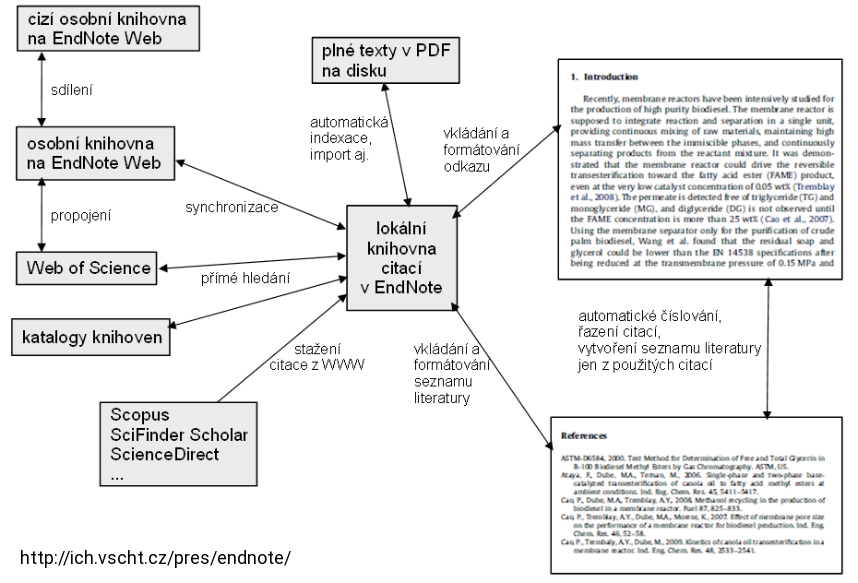
\includegraphics[height=6.5cm]{mapa_funkci.png}
	\end{center}
\end{frame}

\begin{frame}{Stáhnutí citace}
	\begin{itemize}
		\item Většina on-line databází nabízí možnost exportu záznamu v~různých formátech\ldots
		\item Většina programů umí importovat víc formátů\ldots
	\end{itemize}
	\begin{center}
		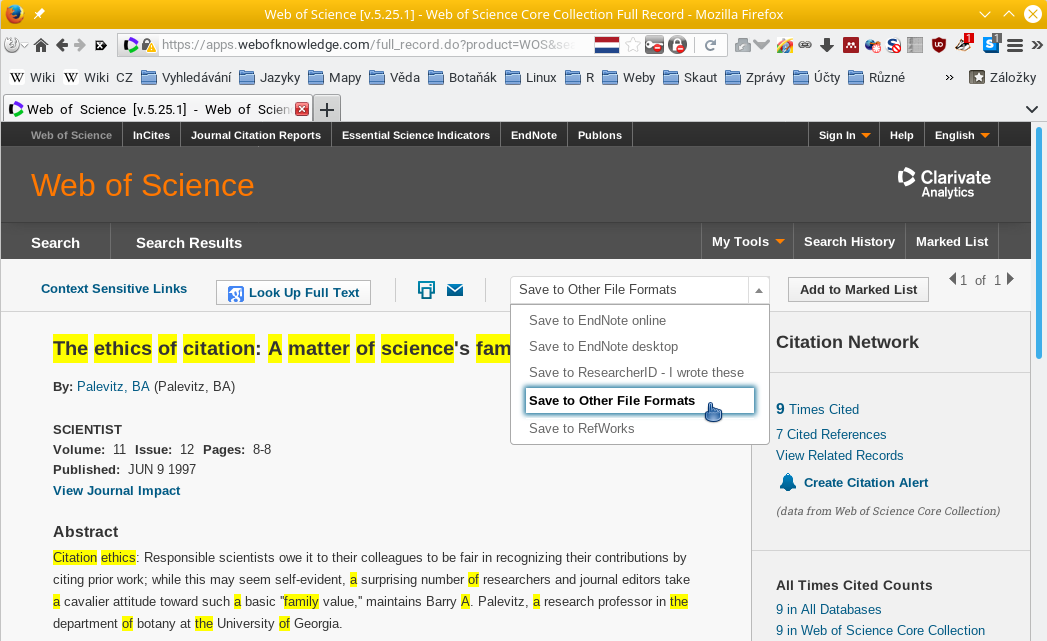
\includegraphics[height=6cm]{export_z_wos.png}
	\end{center}
\end{frame}

\section{Mendeley}

\begin{frame}{Mendeley}
        Dostupný zdarma, multiplatformní, s~možností on-line synchronizace (zdarma 2~GB prostoru, víc lze dokoupit),~\ldots\\
        \begin{center}
                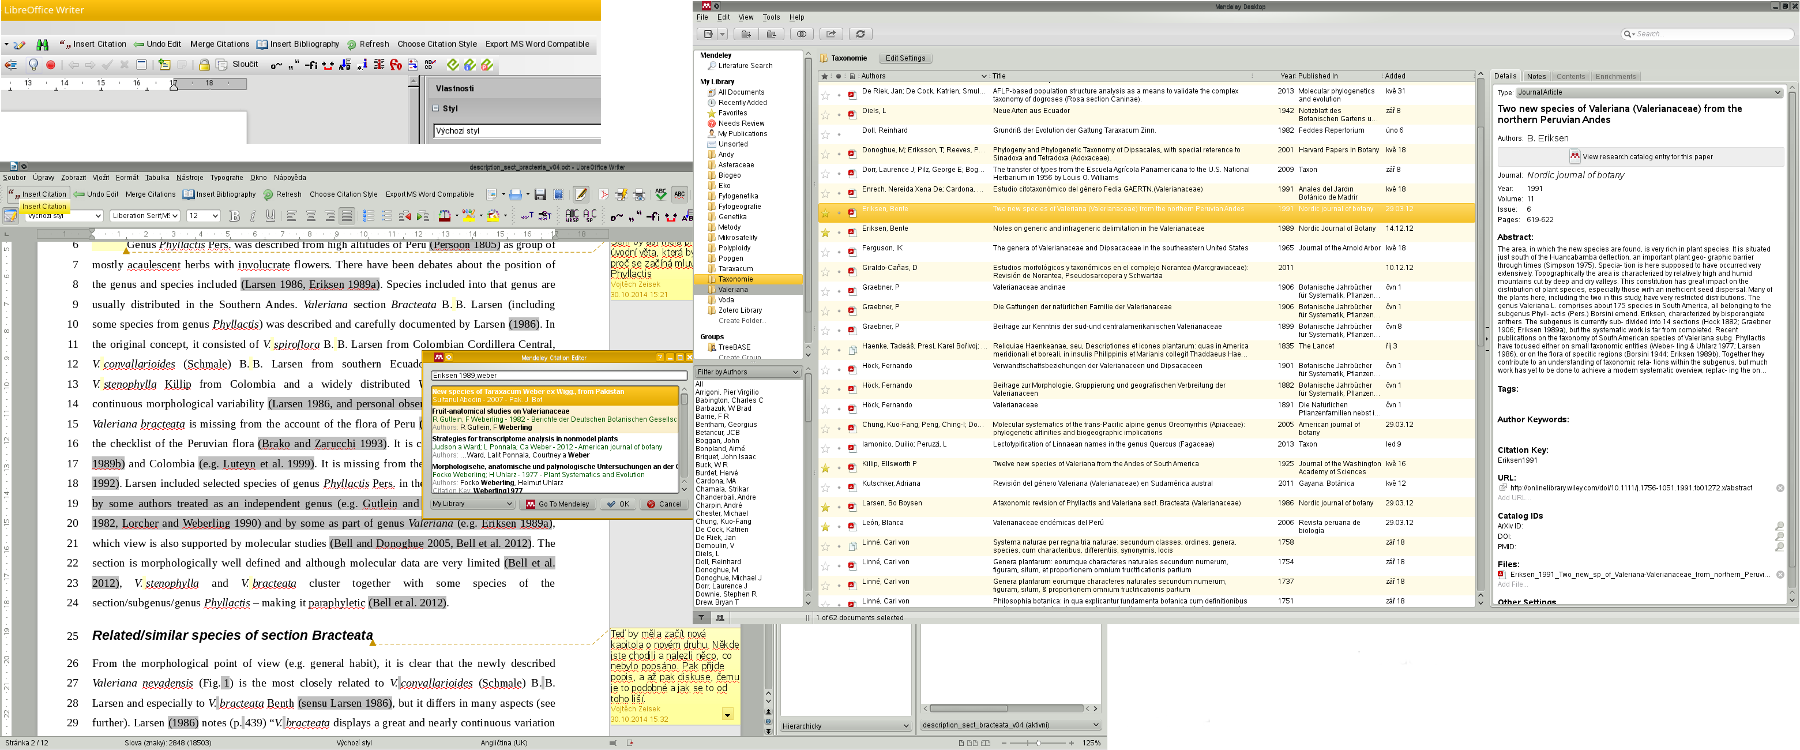
\includegraphics[height=5cm]{mendeley.png}
        \end{center}
        \flushright\url{https://www.mendeley.com/}
\end{frame}

\begin{frame}{Mendeley web}
	\begin{itemize}
		\item Knihovna je dostupná on-line
		\item Články lze prostřednictvím skupin sdílet s~kolegy
		\item Lze prohledávat on-line databáze a~rovnou přidávat do~knihovny
		\item A~další funkce\ldots{ }Ostatní to~mají podobně\ldots
	\end{itemize}
	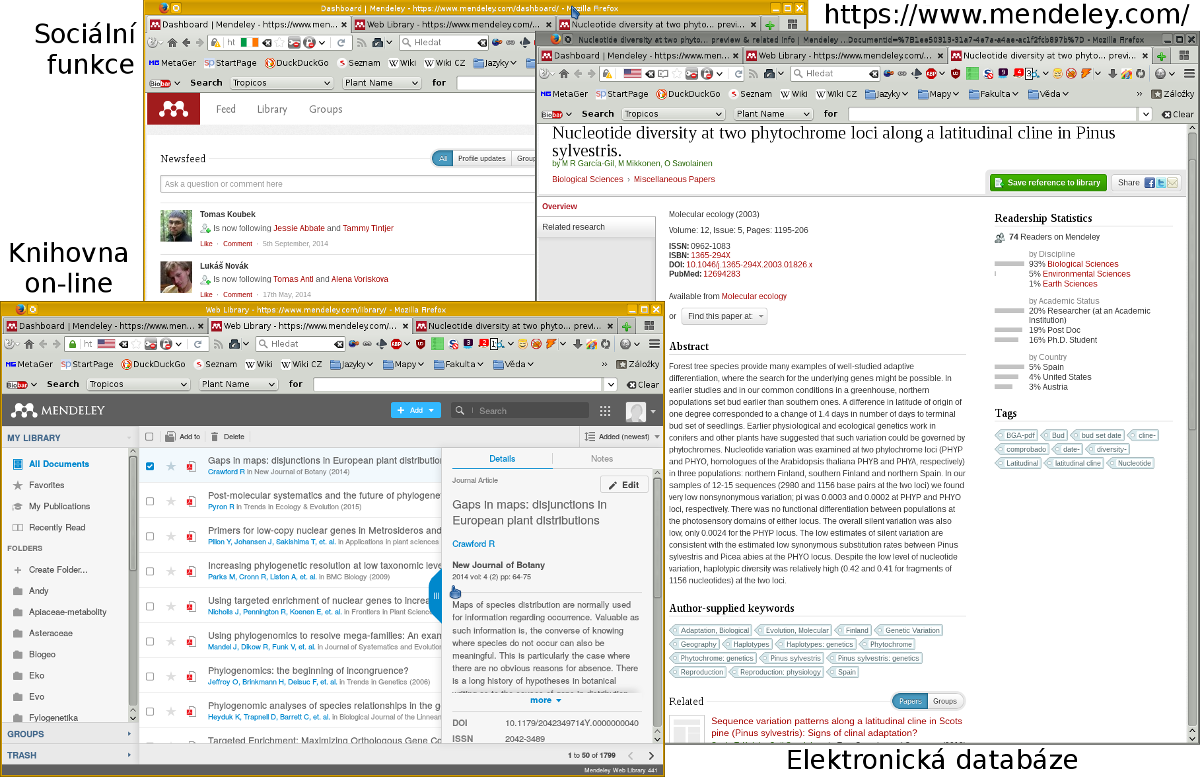
\includegraphics[width=\textwidth]{mendeley_web.png}
\end{frame}

\begin{frame}{Import ze~stránky časopisu do~Mendeley}{Článek se~naimportuje do~on-line knihovny a~z~ní~se~synchronizuje do~aplikace v~počítači}
	\begin{itemize}
		\item Lze importovat z~webových článek časopisů, z~on-line databází, z~PDF článků, z~jiných citačních nástrojů,~\ldots
	\end{itemize}
	\begin{center}
		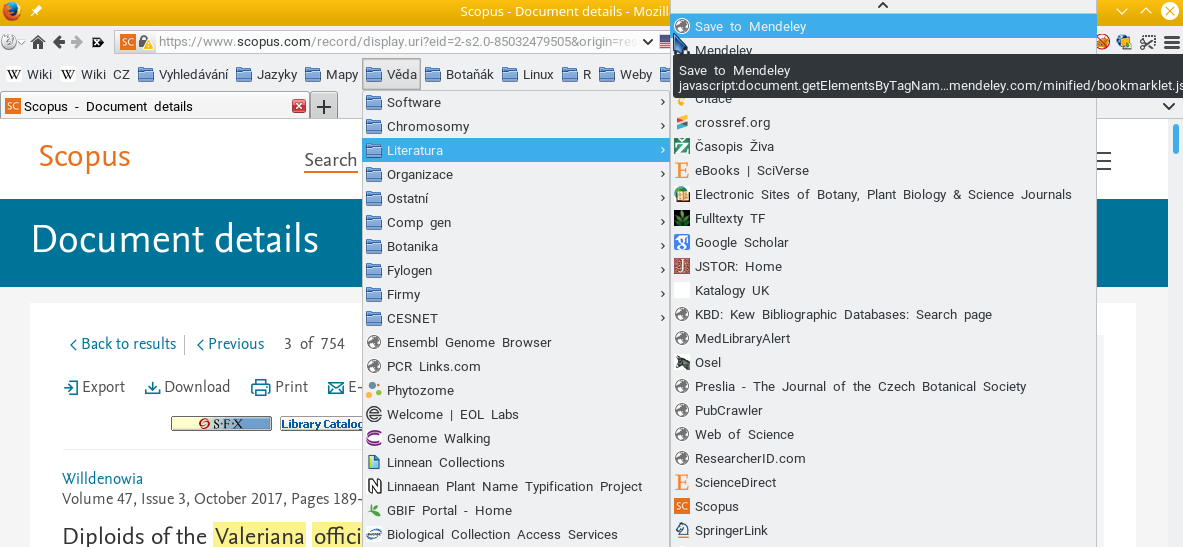
\includegraphics[height=5.5cm]{mendeley_web_import.png}
	\end{center}
\end{frame}

\section{Zotero}

\begin{frame}{Knihovna v~Zoteru}
	\begin{itemize}
		\item Zotero (\url{https://www.zotero.org/}) má doplněk pro~prohlížeč (Mozilla Firefox, Google Chrome a~odvozeniny, Apple Safari a~MS~Edge) a~samostatnou aplikaci pro~MS~Windows, macOS i~Linux
	\end{itemize}
	\begin{center}
		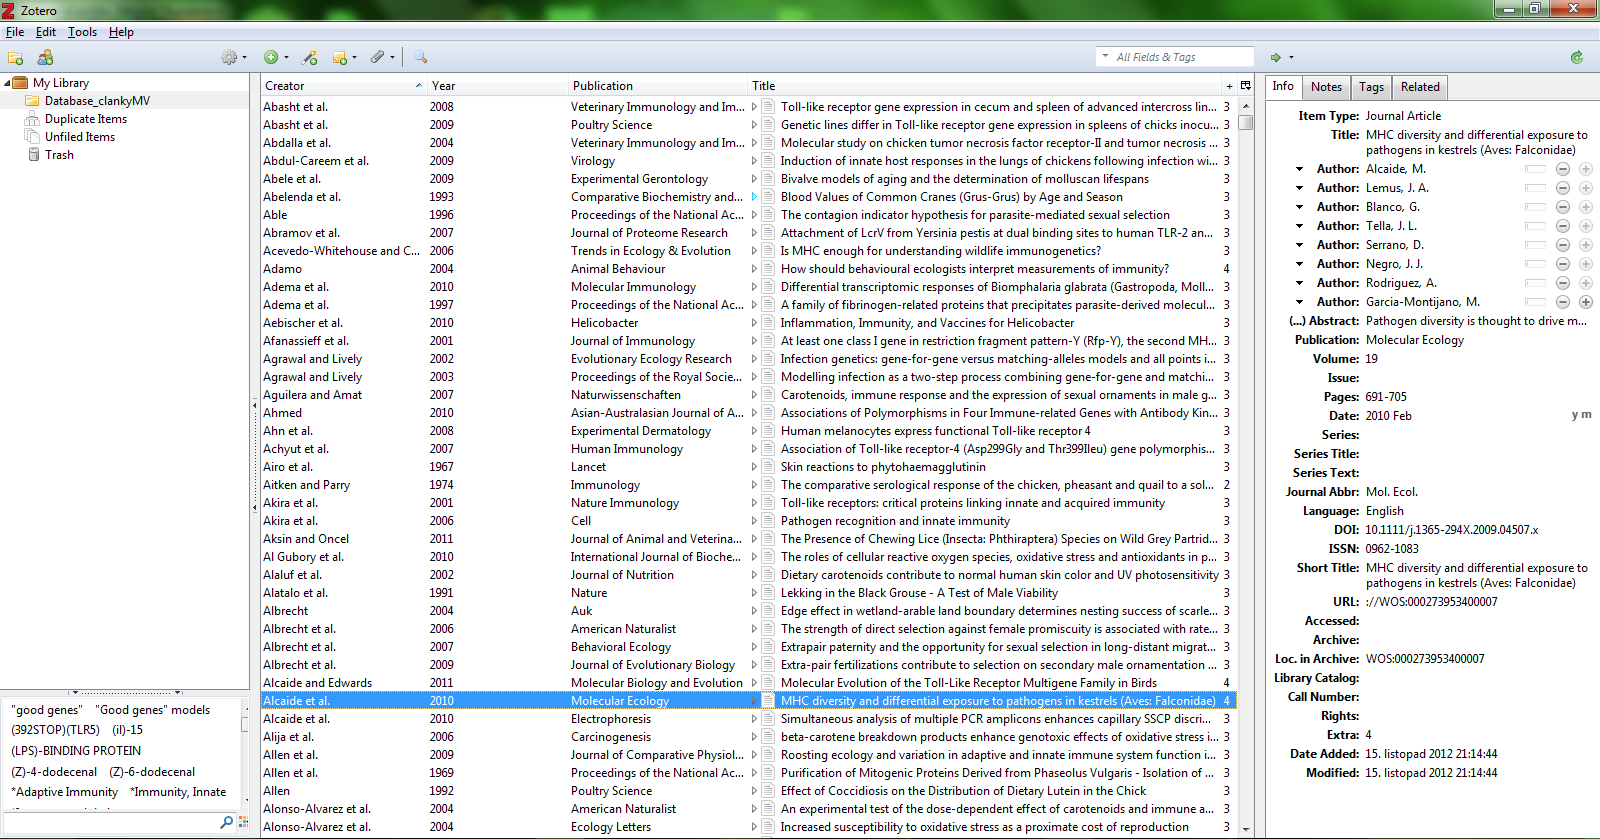
\includegraphics[height=5.5cm]{zotero.png}
	\end{center}
\end{frame}

\begin{frame}{Vkládání do~Wordu nebo podobného programu}
	\begin{itemize}
		\item Zotero a~Mendeley spolupracují s~MS Office i~\href{https://cs.libreoffice.org/}{Libre Office} na~Windows, macOS i~Linuxu, komerční programy obvykle jen s~MS Word na~MS Windows nebo macOS
	\end{itemize}
	\begin{center}
		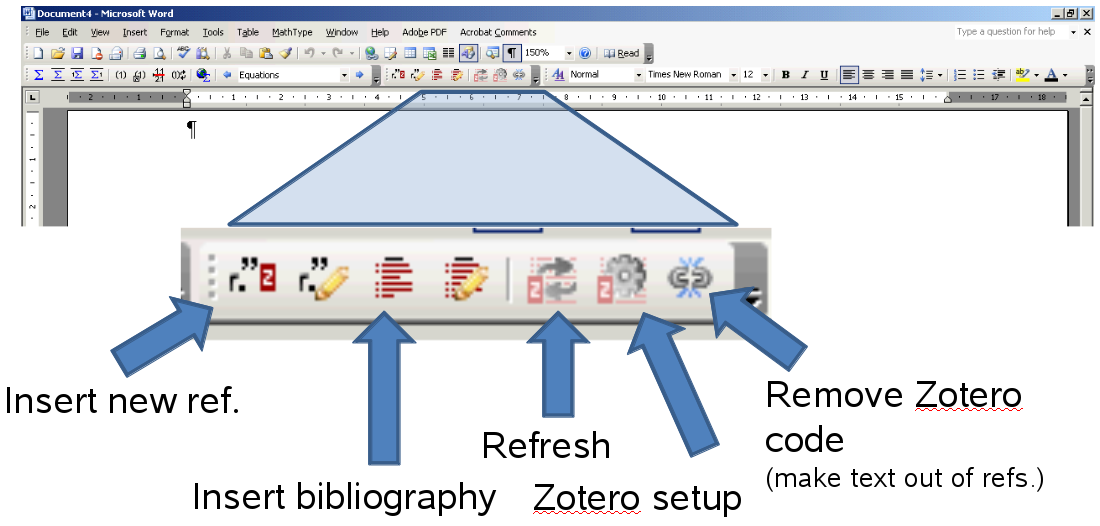
\includegraphics[height=6cm]{zotero_lista.png}
	\end{center}
\end{frame}

\begin{frame}{Praktická ukázka\ldots}{Vkládání a~správa citací ze~Zotera do~textového procesoru}
	\begin{center}
		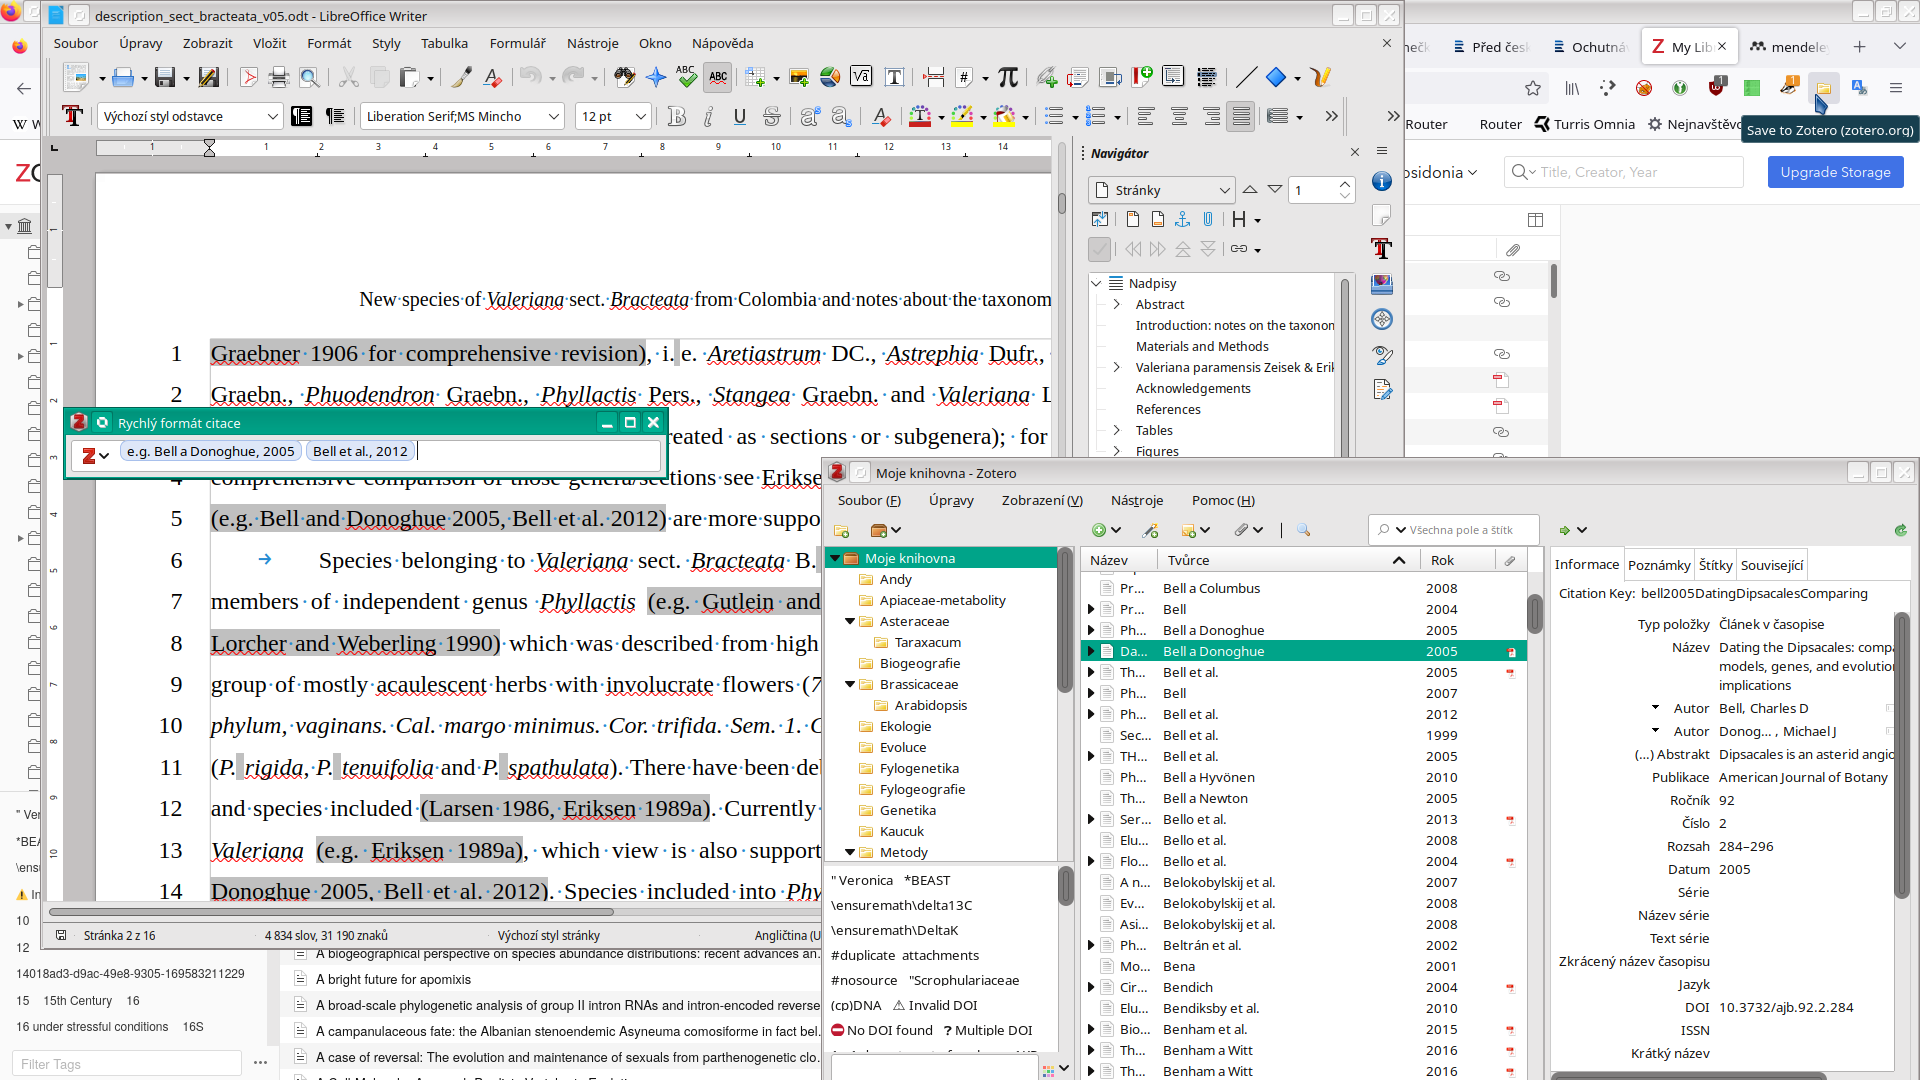
\includegraphics[height=6.5cm]{zotero_writer_knihovna.png}
	\end{center}
\end{frame}

\section{Závěr}

\begin{frame}[allowframebreaks]{Špetka typografie a~usnadnění práce}
	\begin{itemize}
		\item \textbf{Používejte styly!}
			\begin{itemize}
				\item Můžete formát nadpisů, odstavců apod. měnit centrálně --- změny se~ihned projeví všude (ručně vždy někde něco zkazíte\ldots)
				\item Text bude mít jednotný vzhled, styly logicky povedou čtenáře
				\item Ze~stylů nadpisů lze na~pár kliknutí vygenerovat hierarchický obsah (samozřejmě nastylovatelný)
				\item \textbf{Needitujte ručně} vzhledy odstavců, speciálních formátů (pro~zdrojový kód,~\ldots) --- vše řešte přes předdefinované styly
				\item Na~začátku je s~tím víc práce, ale celkově se~to~velmi vyplatí
			\end{itemize}
		\item \textbf{Používejte křížové odkazy a~pole!}
			\begin{itemize}
				\item Slouží jako propojení mezi prvky dokumentu --- typicky jako odkaz na~obrázek apod. (lze odkázat na~jeho různě zformátované číslo, stránku,~\ldots)
				\item Číslování obrázků, tabulek, apod. se~automaticky aktualizuje při~přidání/odebrání/přesunutí, stejně tak~odkazy na~daný obrázek/\ldots
				\item Lze automaticky vygenerovat seznamy obrázků/tabulek/\ldots
			\end{itemize}
		\item Často ukládejte, včetně \href{https://www.natur.cuni.cz/biologie/botanika/provozni-informace/servery-weby-a-pocitace/moznosti-zalohovani-dat}{záloh}, ukládejte různé verze --- můžete se k~něčemu vrátit
		\begin{itemize}
			\item Užitečné je použít nějaký nástroj pro správu verzí --- základní funkce jsou v~Office sadách, pokročilejší uživatelé mohou použít třeba \href{https://git-scm.com/book/cs/v2}{Git} --- v~případě potřeby se~můžete vrátit k~předchozí verzi dokumentu
		\end{itemize}
		\item Seznamte se~se~\href{https://duckduckgo.com/?q=typografick\%C3\%A1+pravidla&ia=web}{základními typografickými pravidly}
		\begin{itemize}
			\item \href{https://cs.wikipedia.org/wiki/Typografie}{Typografie} (grafická úprava textu) slouží k~tomu, aby~se~text dobře (pohodlně) četl (a~zároveň dobře vypadal)
			\item V~odborném textu sjednocuje styl psaní např. jednotek, odborných jmen \textit{kurzívou} apod., což~usnadňuje orientaci v~textu a~odstraňuje nejasnosti při čtení
			\item Pro angličtinu viz např. \href{https://authorservices.wiley.com/author-resources/book-authors/prepare-your-manuscript/house-style.html}{Wiley House Style}
		\end{itemize}
		\item Čtěte nápovědy svých programů
			\begin{itemize}
				\item Ať už~používate cokoliv, používejte to~efektivně
				\item Vaše programy možná (určitě:-) umí víc, než si~myslíte\ldots
				\item Děláte-li ručně nějakou nudnou opakující se~práci, určitě na~to~existuje jednoduchá automatická funkce\ldots
			\end{itemize}
		\item Odkazy na návody
			\begin{itemize}
				\item \href{https://www.linuxexpres.cz/kancelar/jak-vytvorit-zaverecnou-pisemnou-praci}{Jak vytvořit závěrečnou písemnou práci} --- návod původně pro OpenOffice, ale logika je platná pro všechny podobné programy
				\item \href{https://www.root.cz/knihy/libreoffice-writer-prakticky-pruvodce/}{Kniha LibreOffice Writer: Praktický průvodce} --- vše, co~jste potřebovali vědět (starší, ale stále platné)
				\item \href{https://cs.libreoffice.org/get-help/documentation/}{Uživatelská příručky LibreOffice}
				\item \href{https://formatovani-dokumentu.cz/navody}{Návody, formátování,~\ldots}
				\item Ptejte se~svých \href{https://www.startpage.com/}{oblíbených} \href{https://duckduckgo.com/}{vyhledávačů} a/nebo umělé inteligence (vyřeší vám spoustu technických potíží)
			\end{itemize}
		\item Aby text vypadal dobře, je lepší se~vyhnout kancelářským sadám (MS~Office, LibreOffice,~apod.) a~použít raději nástroj specializovaný na~sazbu
			\begin{itemize}
				\item Nejjednodušší je text za~použití stylů napsat v~nějaké Office sadě a~vysázet ve~\textbf{Scribu} (\url{https://www.scribus.net/} a~\url{https://scribus.cz/}, což je program specializovaný na~sazbu, podobně jako \href{https://www.natur.cuni.cz/fakulta/cit/podpora-uzivatelu/softwarove-licence/adobe}{Adobe} InDesign) nebo v~něčem podobném
			\end{itemize}
	\end{itemize}
\end{frame}

\begin{frame}{Užitečné odkazy}
	\begin{itemize}
		\item EndNote: \url{https://endnote.com/}
		\item Zotero: \url{https://www.zotero.org/}
		\item Mendeley: \url{https://www.mendeley.com/}
		\item Tutoriál k~EndNote: \url{http://ich.vscht.cz/pres/endnote/}
		\item Návod na Mendeley: \url{https://www.linuxexpres.cz/software/mendeley-a-mate-poradek-v-publikacich}
		\item Návod na Zotero: \url{https://www.zotero.org/support/quick_start_guide}
		\item \BibTeX{ }a~\XeLaTeX{ }(v~Linuxu): \url{https://www.linuxexpres.cz/software/kile-a-kbibtex}
		\item Vizuální editor pro \XeLaTeX{ }(pro všechny systémy): \href{https://www.linuxexpres.cz/software/textovy-editor-lyx-latex-pro-line}{úvod} a~\href{https://www.linuxexpres.cz/praxe/diplomka-lyx}{podrobnější návod}
	\end{itemize}
\end{frame}

\begin{frame}{Děkuji za pozornost\ldots}
	\begin{Large}
		\begin{flushright}
			\ldots otázky?
		\end{flushright}
	\end{Large}
	\begin{center}
		
\includegraphics[height=5cm]{phdcomics_writing.png}
	\end{center}
	\begin{flushright}
		\begin{scriptsize}
			\url{https://phdcomics.com/comics/archive.php?comicid=1732}
		\end{scriptsize}
	\end{flushright}
	\begin{tiny}
		Vysázeno v~\XeLaTeX u~na \href{https://www.opensuse.org/}{openSUSE GNU/Linuxu} \today.
	\end{tiny}
\end{frame}

\end{document}

